\section{Design}

\begin{figure}[t]
    \centering
    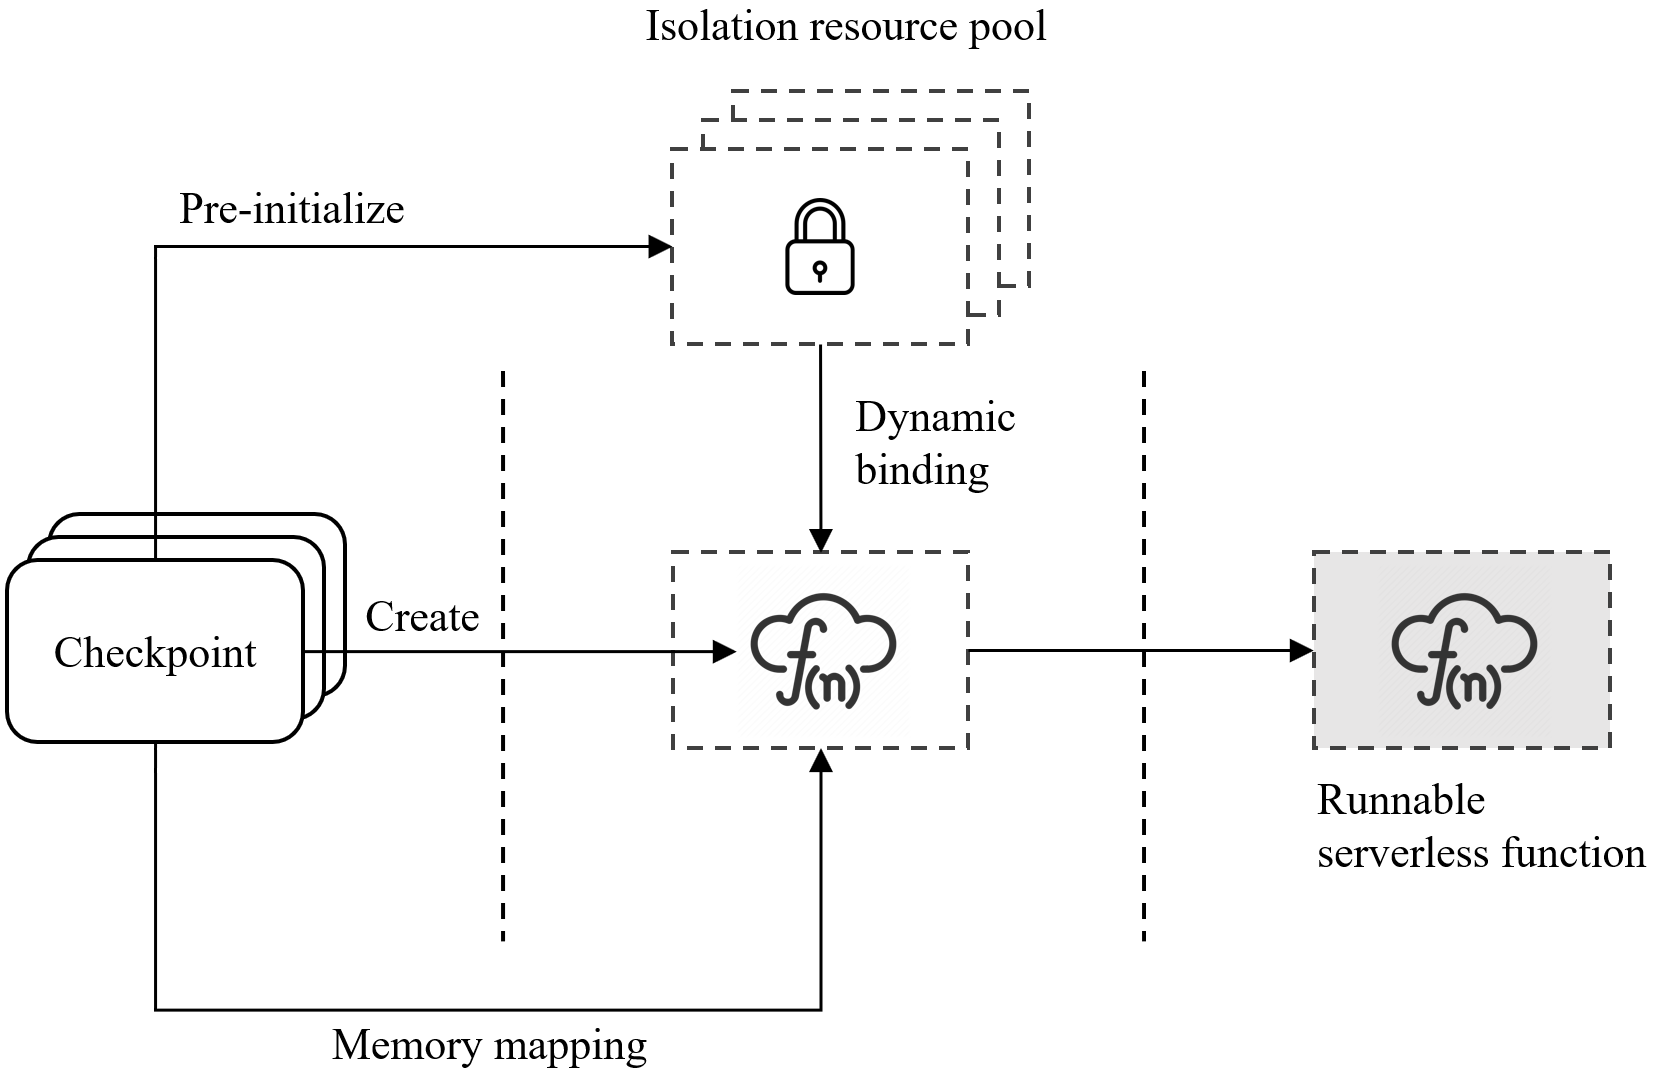
\includegraphics[width=\linewidth]{images/design.PNG}
    \caption{Overview of ProjectName}
    \label{design}
\end{figure}

In this paper we propose \pname, 
which is mainly based on CRIU, 
and uses multiple optimization mechanisms to effectively reduce the complexity of the restoration process of serverless functions, 
providing a stable and better startup performance.


As shown in the figure \ref{design}, 
before starting the function, 
\pname will use the information recorded in the function checkpoint to \textit{pre-initialize} 
multiple namespace resources required to build the sandbox environment, 
which constitutes the \textit{isolated resource pool}.
When \pname receives the request to start the function and creates the function process, 
it will \textit{dynamically bind} the function process and the matching namespace resource to speed up the construction of the sandbox environment. 
Then \pname restores the function memory data through \textit{memory mapping}, 
and finally produces a \textit{runnable serverless function}.

\subsection{Isolation Environment Pooling}
Since the Linux namespace can exist independently of the process, 
that is, 
as long as the file descriptor of the corresponding namespace is opened or bind-mounted to another location, 
even if the process inside the namespace exits, 
the namespace is still valid, 
and other processes can use system calls such as setns to enter the namespace and modify the related resources referenced by it. 
Based on this feature, we propose an isolation environment pooling strategy for the construction of the function isolation environment.

The strategy creates multiple brand new Mount, UTS, and IPC namespaces in the system before the serverless function starts. 
The newly created namespace cannot be used to assemble the serverless function. Therefore, the strategy needs to parse the checkpoint of each serverless function and initialize each namespace according to the information inside the checkpoint. 
For example, for Mount namespace, 
the function checkpoint contains the mounting information of each filesystem and device in the namespace. 
Using information from the checkpoint, 
the pooling strategy will mount the corresponding filesystem or device to the correct directory location through the recorded mounting parameters; 
for UTS namespace, 
The pooling strategy sets the correct host name and domain name of the container; 
for the IPC namespace, 
relevant core parameters are set  
and structures such as shared memory, 
message queues, and semaphores are created and initialized. 
Through this strategy, 
CRIU does not need to initial Mount, UTS, and IPC namespace again when starting the serverless function, 
but only needs to enter the prepared isolation environment through the setns system call. 

The isolation environment pooling strategy 
essentially removes the function isolation environment 
initialization phase from the startup process and places it to the offline, 
which can greatly reduce the latency in the isolation environment 
initialization phase under the premise of extremely low resource consumption. However, 
this scheme has certain security risks. 
Because the \textit{/proc} directory of the root filesystem provided by the container is attached by the \textit{proc filesystem}, at the same time, 
multiple subdirectories under the \textit{/proc} directory are read-only bind-mounted to prevent the container process from modifying the contents of the directory, which ensures the security of the host. 
The contents of the files and directories contained in the \textit{proc filesystem} are directly related to the PID namespace of the process that mount the \textit{proc filesystem}. 
For example, 
the \textit{/proc/[pid]} subdirectories in the \textit{proc filesystem} only expose the information of all processes in the same PID namespace. 
If the isolation environment pooling strategy is adopted, 
the Mount namespace used by the serverless function will be initialized, 
and the component or system that implements the strategy will use a process to 
attach \textit{/proc} directory with \textit{proc filesystem}, 
which causes the inconsistency between the process that mount the \textit{proc filesystem} and the process ultimately running in this namespace. 
If the function process use the pre-initialized Mount namespace directly, 
it will bring security risks of host data leakage, 
which may cause the function to exit, 
or damage the security of the container environment.

\begin{figure}[t]
    \centering
    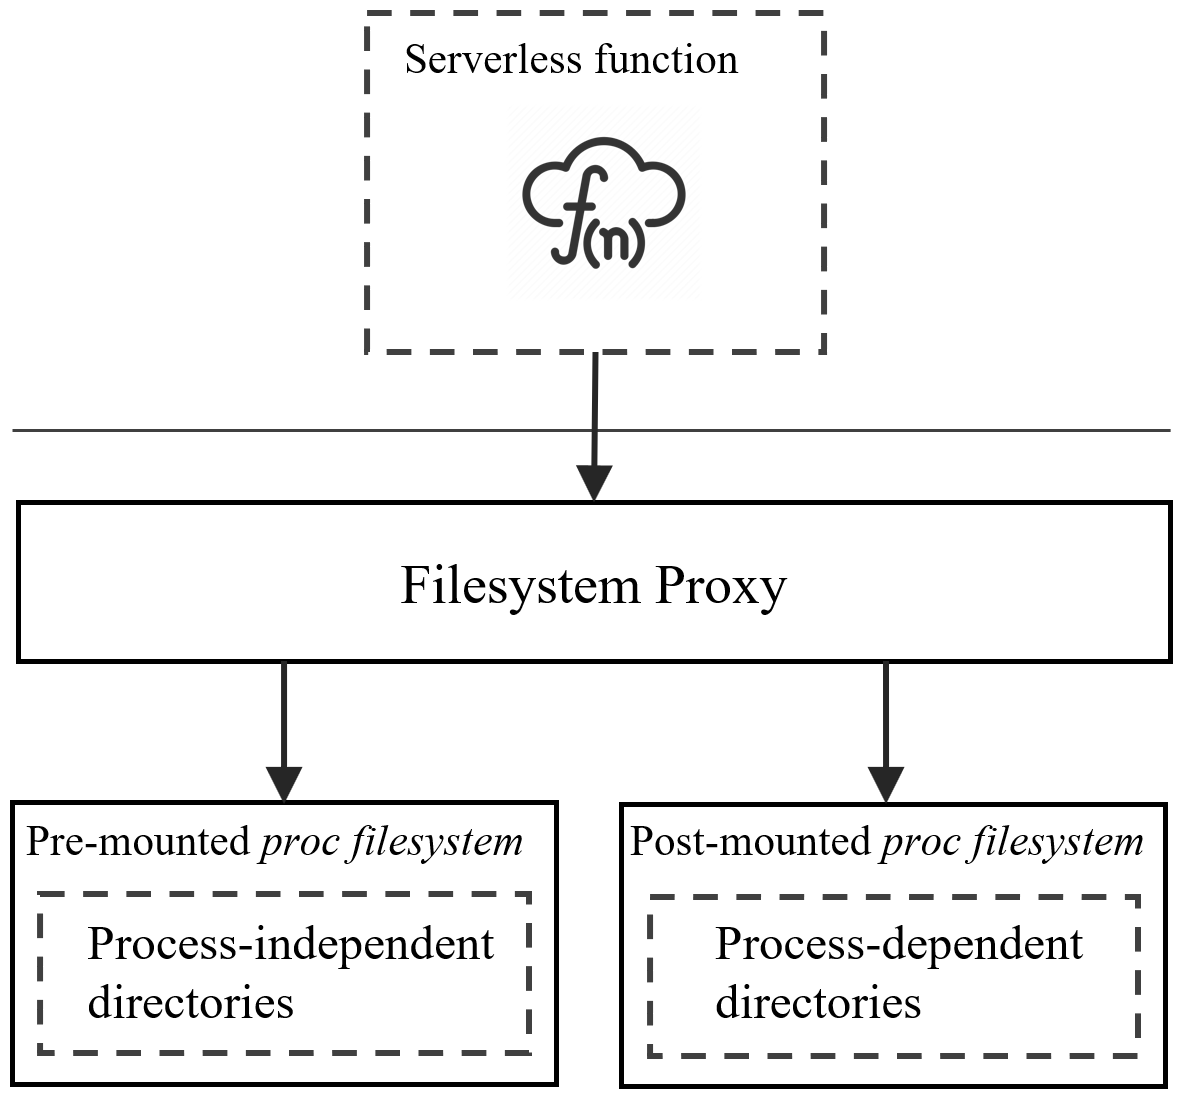
\includegraphics[width=2.5in]{images/fs-proxy.PNG}
    \caption{Filesystem proxy}
    \label{fs-proxy}
\end{figure}
In order to avoid the introduction of the aforementioned systemic risks and ensure the efficiency of function startup, 
\pname introduces the \textit{filesystem proxy} 
which forwards requests from processes in the container to access the /proc directory. 
As shown in the figure \ref{fs-proxy}, 
There are two types of \textit{proc filesystem} below the \textit{filesystem proxy}. 
One is the \textit{"pre-mounted proc filesystem"} which is mounted through the isolation environment pooling strategy, 
the other is the \textit{"post-mounted proc filesystem"} that is simply mounted by the container process when the container starts. 
When a serverless function accesses the \textit{/proc} directory, 
it will first access the \textit{filesystem proxy} layer. 
The \textit{filesystem proxy} will judge the specific directory to be accessed. 
If the directory to be accessed containes content that has nothing to do with the process PID namespace, 
the access request will be forward to the \textit{"pre-mounted filesystem"}, 
otherwise the \textit{filesystem proxy} will synthesize the contents of the corresponding directory of the \textit{"post-mounted proc filesystem"} 
and the access attributes of the corresponding directory of the \textit{"pre-mounted proc filesystem"} to give a correct response. 
Using the \textit{filesystem proxy strategy} to forward access requests not only ensures the effectiveness of the pooling strategy, 
but also prevents the security of the container environment from being weakened.

\subsection{Function Memory Shared Mapping}
\begin{figure}[t]
    \centering
    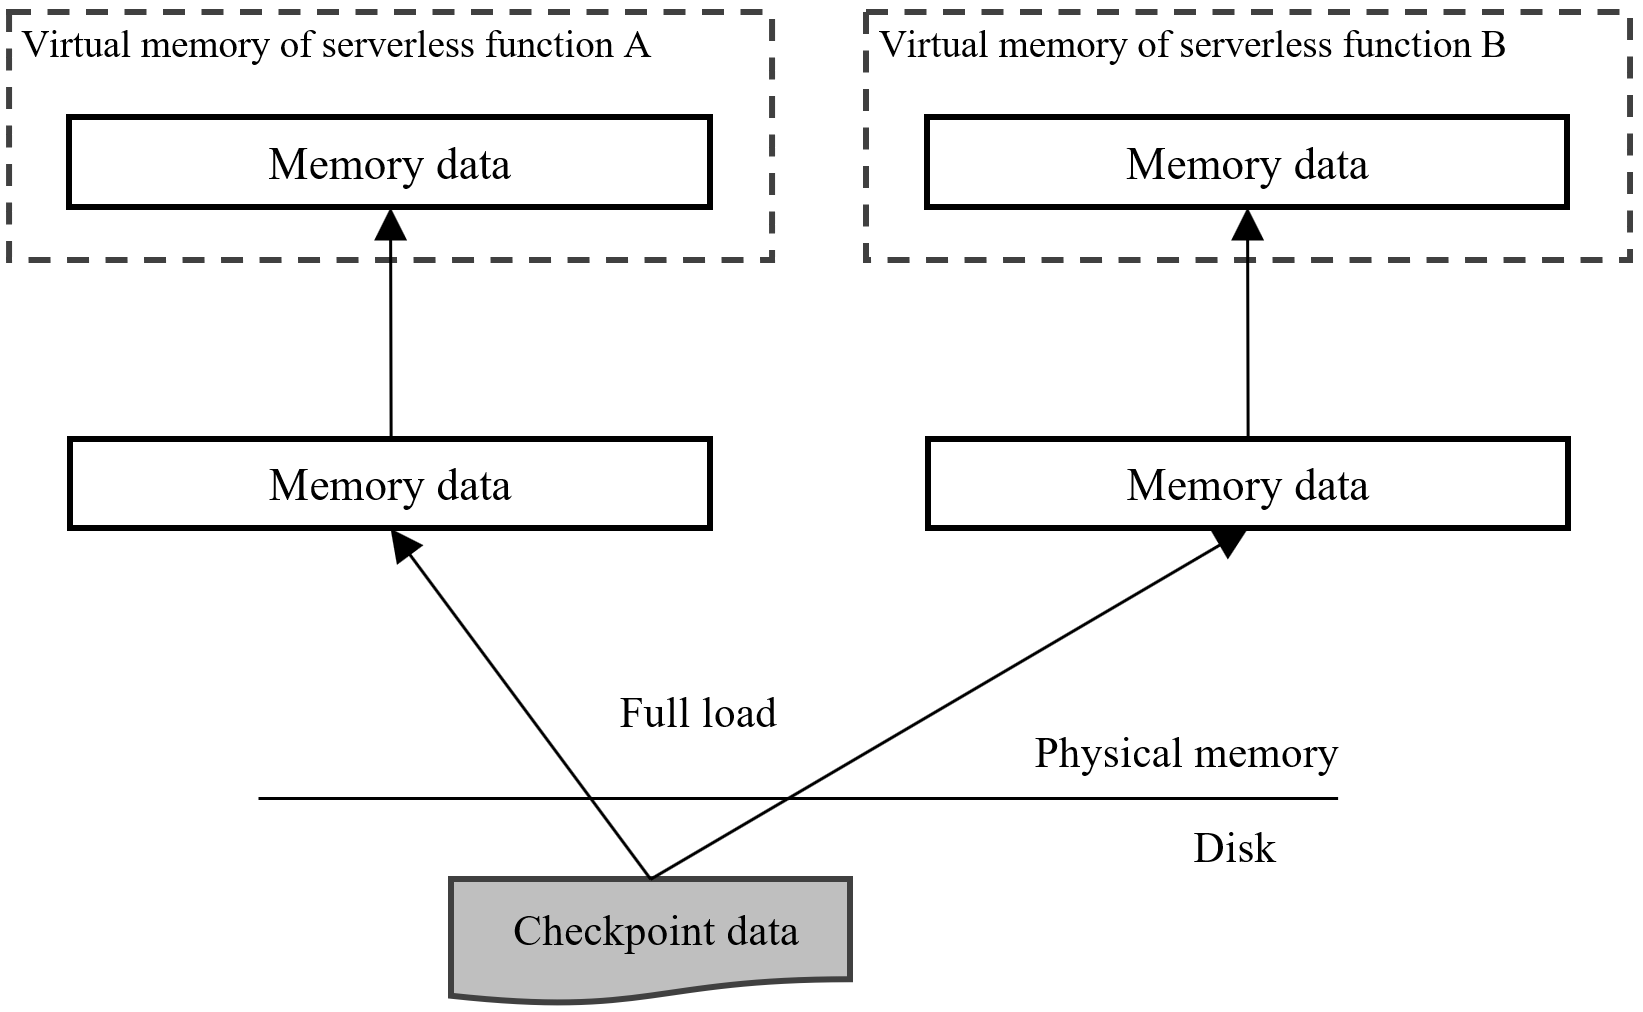
\includegraphics[width=\linewidth]{images/full-load-memory.PNG}
    \caption{Memory data redundancy brought by multiple identical serverless functions}
    \label{full-load-memory}
\end{figure}

As shown in the figure \ref{full-load-memory}, 
CRIU uses a full-load method when restoring the function memory data, 
which copies the memory page data from the checkpoint to the corresponding location in the process's virtual memory space. 
For serverless functions that require a large amount of memory in runtime, the checkpoint contains more memory data. 
Since the reading of the checkpoint is essentially a reading to the disk, 
it brings quite high latency. 
At the same time, 
the full-load method results in multiple copies of the same data in the physical memory. 
Even if the memory data of multiple identical serverless functions are basically the same, 
because the memory data cannot be shared between function processes, 
memory data redundancy occurs, 
which severely reduces the resource utilization of the platform.

\begin{figure}[t]
    \centering
    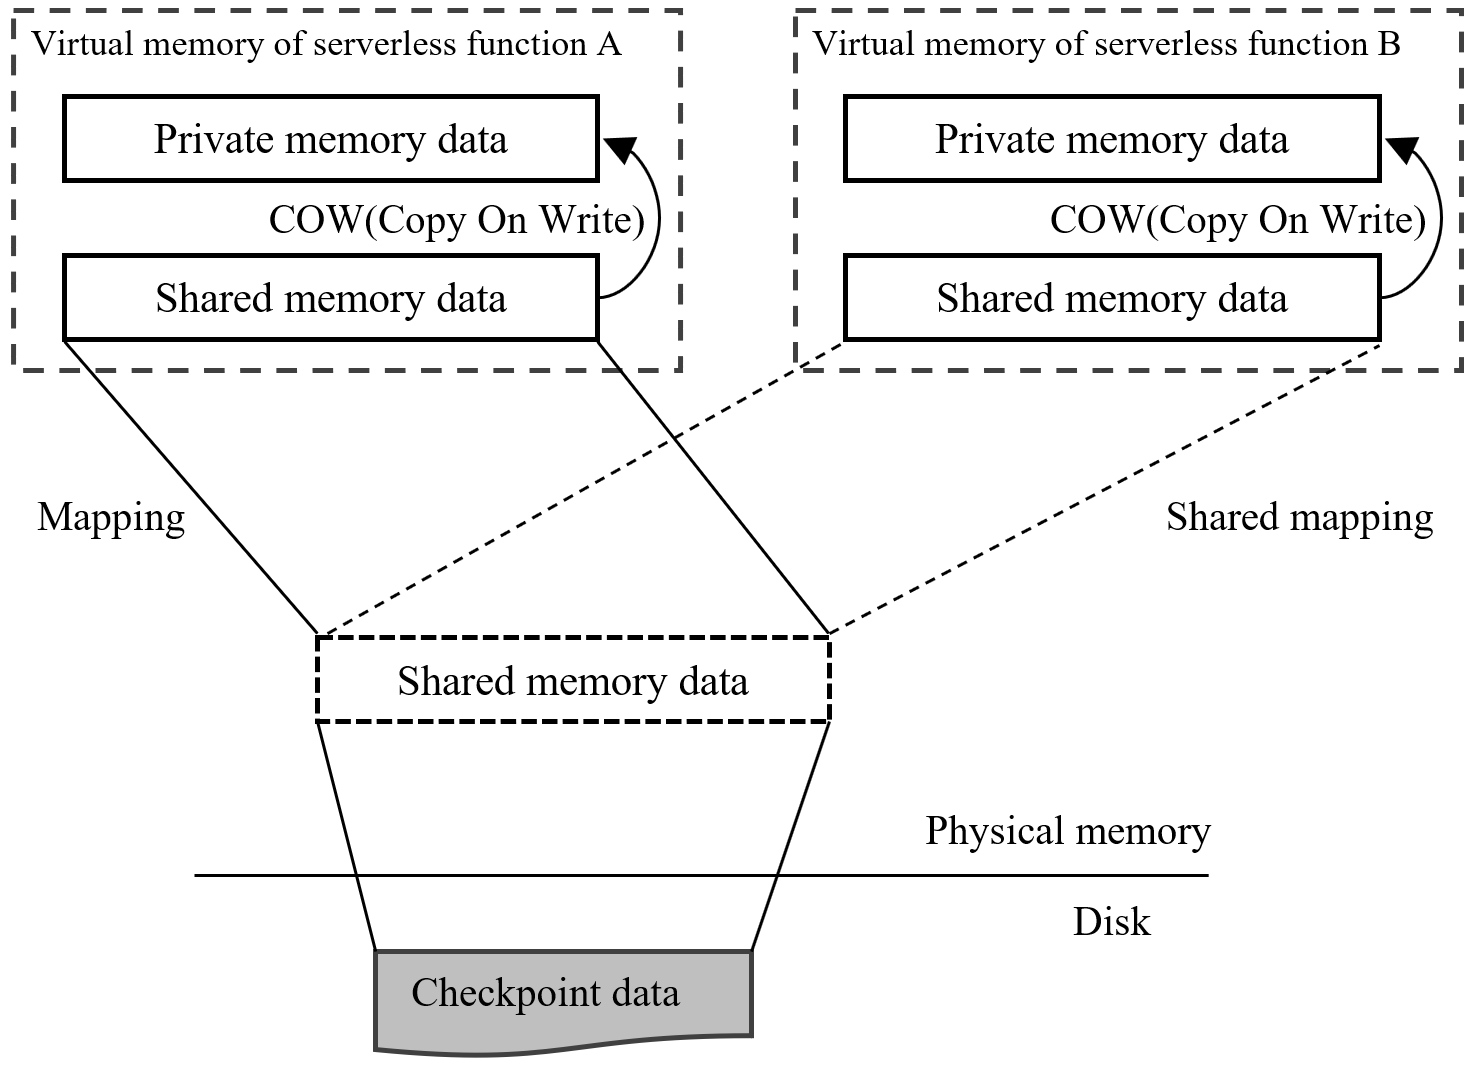
\includegraphics[width=\linewidth]{images/shared-memory.PNG}
    \caption{Function memory shared mapping}
    \label{shared-mapping}
\end{figure}

This paper introduces the shared mapping strategy 
of function's memory to replace the original memory restoration method of CRIU. 
As shown in the figure \ref{shared-mapping}, 
the CRIU restores the memory data of serverless functions by 
establishing the mapping relationship between the virtual memory space 
of the function process and the corresponding memory page in the checkpoint. 
This mapping does not lead to the reading of the memory data. 
Only when the serverless function accesses the mapped virtual memory space during the startup, 
the corresponding data in the checkpoint will be loaded into the physical memory.
This memory restoration method allows the memory data in the checkpoint to be loaded into the physical memory on demand, which greatly reduces the delay of the restoration of the memory data, and avoids temporarily unnecessary data from being copied to the physical memory prematurely, 
causing a waste of system resources.

At the same time, 
the mapping method allows multiple serverless 
functions started from the same checkpoint to share the same physical memory space, 
avoiding the waste of resources when a serverless computing application is deployed on a node on a large scale. 
As shown in the figure \ref{shared-mapping}, 
the memory pages mapped into the virtual memory space of the function process are all read-only. 
When the function process tries to modify the data of a certain memory page, 
the \textit{Copy on Write(COW)} mechanism of the operating system  
will make a copy of the page for private write operations.